% Notes for Aulas 1-2 of Economia das Organizacoes e dos Incentivos (MPE Insper).
% Compile: pdflatex main.tex (twice). Check: pdffonts main.pdf (all Type 1, uni = yes).
\documentclass[11pt,a4paper]{article}
\usepackage[utf8]{inputenc}
\usepackage[T1]{fontenc}
\usepackage{lmodern}   % Type 1 vector fonts (replaces PK bitmaps)
\usepackage{cmap}      % ToUnicode CMap -> copyable text and accents
\usepackage[english]{babel}
\usepackage{amsmath,amssymb,amsthm,mathtools}
\usepackage[a4paper,margin=2.4cm]{geometry}
\usepackage{microtype}
\usepackage{booktabs,tabularx,array}
\usepackage{enumitem}
\usepackage{xcolor}
\usepackage{tikz}
\usetikzlibrary{arrows.meta,calc,patterns}
\usepackage{pgfplots}
\pgfplotsset{compat=1.17}
\usepackage[most]{tcolorbox}
\usepackage{fancyhdr}
\usepackage[hidelinks]{hyperref}

\setlist{topsep=3pt,itemsep=2pt}
\setlength{\parindent}{0pt}
\setlength{\parskip}{5pt}
\renewcommand{\arraystretch}{1.2}

\pagestyle{fancy}\fancyhf{}
\lhead{\footnotesize Economics of Organizations and Incentives --- MPE Insper}
\rhead{\footnotesize Notes, Aulas 1--2}
\cfoot{\footnotesize\thepage}
\renewcommand{\headrulewidth}{0.3pt}
\setlength{\headheight}{14pt}

\definecolor{defc}{RGB}{30,80,150}
\definecolor{propc}{RGB}{110,40,130}
\definecolor{exc}{RGB}{20,110,70}
\definecolor{warnc}{RGB}{170,60,30}

% Boxes. \begin{defn}{Title} ... \end{defn}; same for prop, example, keyidea, caution.
\newtcolorbox{defn}[1]{enhanced,breakable,colback=defc!4,colframe=defc,
  fonttitle=\bfseries,title={Definition: #1},left=6pt,right=6pt}
\newtcolorbox{prop}[1]{enhanced,breakable,colback=propc!4,colframe=propc,
  fonttitle=\bfseries,title={#1},left=6pt,right=6pt}
\newtcolorbox{example}[1]{enhanced,breakable,colback=exc!4,colframe=exc,
  fonttitle=\bfseries,title={Example: #1},left=6pt,right=6pt}
\newtcolorbox{keyidea}{enhanced,breakable,colback=gray!6,colframe=gray!60,
  boxrule=0.4pt,left=6pt,right=6pt,fontupper=\itshape}
\newtcolorbox{caution}[1]{enhanced,breakable,colback=warnc!4,colframe=warnc,
  fonttitle=\bfseries,title={#1},left=6pt,right=6pt}

\newcommand{\MR}{M\&R}
\newcommand{\pg}[1]{(p.~#1)}          % printed page of M&R unless another book is named
\newcommand{\R}{\mathbb{R}}
\DeclareMathOperator*{\argmax}{arg\,max}

\title{\textbf{Does Organization Matter? and Bargaining}\\[4pt]
  \large Notes for Aulas 1--2 --- Economics of Organizations and Incentives (MPE Insper)}
\author{Built on Milgrom \& Roberts (1992), with Cabral (2017), Varian (2014, with Calculus)\\
  and Mas-Colell, Whinston \& Green (1995)}
\date{October 2026}

\begin{document}
\maketitle
\thispagestyle{empty}

\begin{abstract}
\noindent Part I reads the Ford, GM and Toyota cases as answers to the two problems every
organization faces, coordination and motivation, and then gives the mathematics of fit:
complementarities, coherent systems, and the valley between them. Part II asks what bargaining
decides. Under no wealth effects and complete information, the value maximization principle and
the Coase theorem make the value-creating choice determinate, and bargaining power only divides
the gains (Nash, Rubinstein). Private information breaks this: efficient trade can become
infeasible, and incentive-efficient arrangements give up the small gains. Page numbers are
Milgrom \& Roberts' printed pages unless another book is named. Every worked example is original;
book exercises are cited by number and page only.
\end{abstract}

\tableofcontents
\newpage

\part{Aula 1 --- Does Organization Matter? Ford $\times$ GM $\times$ Toyota}
% Part I: Aula 1 --- Does Organization Matter? Ford x GM x Toyota.
% Converted from Aula/aula-01-notes.md. Numbers checked against the md's formulas in Python
% (n_s = 1.5625, valley 83.926 at n_s; A = 30: 105.917 and 88.389; cube corners and orders).

\textbf{Syllabus item.} \emph{Aplicação: As organizações importam? Ford x GM x Toyota} (Topic 1).
\textbf{Read.} Milgrom \& Roberts (1992), Ch.~1 ``Does Organization Matter?'' (pp.~2--18);
Ch.~4 ``Coordination and Business Strategy'' (pp.~106--113); Cabral (2017) \S3.5 ``Why are firms
different?'' (pp.~56--59).

Page numbers are \MR's printed pages unless another book is named. Facts that do not come from
\MR\ carry their source inline; the stylized numbers are illustrative and checked by
\texttt{aula-01-companions/check\_companions.py} and the video's \texttt{check\_numbers.py}.
Three interactive companions in \texttt{Aula/aula-01-companions/} illustrate the formal part:
\texttt{two\_systems.html}, \texttt{valley.html} and \texttt{multiplier.html}.

% ---------------------------------------------------------------------------------------------
\section{The question}\label{sec:a1-question}

Ford had the technology, the scale and the cost advantage. GM beat it. Toyota was small, short of
capital and technologically behind. It beat GM. \MR's answer, which this class builds up to:

\begin{quote}
``organization and business strategy can be as important as technology, cost, and demand in
determining a firm's success'' \pg{16} --- and what matters most is ``the match of their
strategies and their structures'' \pg{16}.
\end{quote}

The class has two halves. First the cases, read as answers to two problems every organization
faces, \textbf{coordination} and \textbf{motivation} \pg{17}. Then the mathematics of
\textbf{fit}: complementarities, why they make good systems coherent, and why coherent systems are
hard to change one piece at a time.

% ---------------------------------------------------------------------------------------------
\section{Ford: one product, one system}\label{sec:a1-ford}

\MR's picture of Ford is short and exact: ``producing a single product (the Model T Ford) in
high-volume factories using specialized equipment and rigidly disciplined labor paid according to
the job being done'' \pg{109}. It was ``an entirely different but equally coherent strategy that
was appropriate for its time'' and it took Ford past 50\% of the US car market \pg{109}. By 1921
the Model T held \textbf{55\%} of the market, against \textbf{4\%} for Chevrolet and \textbf{11\%}
for all GM brands together \pg{2}.

The pieces, and why each raised the value of the others:

\begin{center}
\small
\begin{tabularx}{\linewidth}{@{}>{\raggedright\arraybackslash}p{0.27\linewidth}
  >{\raggedright\arraybackslash}X >{\raggedright\arraybackslash}X@{}}
\toprule
Choice & What it did & What it needed from the rest \\
\midrule
One model, one colour & long, identical runs & a buyer who wanted a cheap standard car \\
Dedicated machines, moving line & labour per car collapsed & huge, steady volume \\
Narrow, repetitive tasks & unskilled labour could be used & close supervision, a pay premium to
  keep workers \\
High wage (the $\$5$ day, 1914) & turnover fell & the productivity of the line to pay for it \\
Making its own parts & scale in components & the single design \\
\bottomrule
\end{tabularx}
\end{center}

History outside \MR\ (sources in
\texttt{Videos/\allowbreak aula-01-does-organization-matter/\allowbreak provenance.md}): the Model T sold for about
$\$850$ in 1908 and about $\$260$ by the mid-1920s; the moving chassis line (1913) cut assembly
time from about 12.5 hours to 93 minutes by early 1914; 1913 labour turnover was 370\% before the
$\$5$ day (Raff \& Summers 1987; the turnover figures are marked \emph{to confirm} there). The wage
story is efficiency wages, \MR\ Ch.~8 \pg{250}, outside this course's core.

\textbf{The weakness was the same as the strength.} Ford's 1920 answer to the recession was a price
cut of about 25\%, which GM, with higher costs, could not match \pg{2}. Cost leadership worked
while buyers wanted the same car. It stopped working when they wanted different cars.

% ---------------------------------------------------------------------------------------------
\section{GM: variety, and the organization it demanded}\label{sec:a1-gm}

Sloan took over a GM in crisis in 1921: unsold inventories piling up, sales down 75\% between
summer and fall 1920, divisions ``competed mostly with one another'' (pp.~2--3).

\textbf{Strategy.} A car ``for different segments of the market'': Cadillac at the top, each
division a lower-income segment, Chevrolet below the Model T's price \pg{3}.

\textbf{Why the strategy required a new organization.} Variety multiplied the decisions: new
designs, dealers, market information per segment, separate factories and supplies. At the same time
the divisions had to be coordinated: not compete too much, share ideas, coordinate R\&D,
standardize parts ``enough to achieve economies of scale in parts production'' \pg{3}. Neither
Ford's centralized one-product organization nor the old GM, ``a collection of car companies and
suppliers operating without any central direction'', could do this \pg{3}. The old accounting
system had not even charged divisions for the inventories they built up, so they kept producing
into the recession \pg{3}.

\textbf{The multidivisional form} \pg{3}:
\begin{itemize}
  \item divisions keep operating autonomy, each with its own management team and market segment;
  \item a strong central office does \emph{not} run day-to-day operations; it audits and evaluates
    divisions, plans and coordinates strategy, and keeps research, legal and financial functions;
  \item the centre checks internal accounting prices against market prices, so supply divisions
    can be judged ``as if each were a separate firm'' \pg{4}.
\end{itemize}

Henry Ford mocked the ``great big chart'' where a message takes six weeks to travel \pg{4}. The
result: from 1927 to 1937 Ford lost $\$200$ million and GM earned over $\$2$ billion; by 1940 GM
had 45\% of the market, Ford 16\% \pg{4}.

\textbf{GM's system fit together too.} Shared components across models let GM afford specialized
equipment for chassis, engines and brakes \pg{5}; its volumes fully used efficient parts plants, so
it integrated vertically \pg{5}, and it made suppliers compete on price \pg{6}. The price of
specialization: major redesigns only about every 12 years in the 1950s and 1960s \pg{5}.

% ---------------------------------------------------------------------------------------------
\section{Toyota: small, poor, and coherent in the other direction}\label{sec:a1-toyota}

Early-1950s Toyota had a ``drastic lack of capital'' and a scale too small to match US costs
\pg{4}. It first tried to copy mass production, then built a different system under Eiji Toyoda and
Taiichi Ohno \pg{4}.

\begin{center}
\small
\begin{tabularx}{\linewidth}{@{}>{\raggedright\arraybackslash}p{0.27\linewidth}
  >{\raggedright\arraybackslash}X >{\raggedright\arraybackslash}X@{}}
\toprule
Practice (\MR\ pp.~4--6) & Why it followed from Toyota's position & What it then required \\
\midrule
\textbf{Just-in-time / kanban}: no buffer inventories & inventory systems have large scale
  economies Toyota could not reach & every step reliable; defects caught at once \\
\textbf{Operators maintain and repair their own machines} & without buffers, a breakdown stops
  everything & broader skills, authority on the floor \\
\textbf{Flexible equipment}, quick resets, robots by the 1960s & too small to dedicate machines to
  one model & frequent model changes became cheap: redesign twice as often as GM \\
\textbf{Outside suppliers for complex components} & could neither reach efficient scale in parts
  nor afford to own parts makers & close day-to-day coordination with suppliers \\
\textbf{Few suppliers, long-term relations} & high-level components that must fit, frequent
  redesigns & suppliers willing to invest in Toyota-specific skills and machines \\
\bottomrule
\end{tabularx}
\end{center}

\MR's summary of the logic: ``If low inventories were to be achieved, the rest of the organization
had to emphasize reliability, quick response to machine breakdowns, quick and close communications
with suppliers, stable production plans, and other features that substitute for the buffer function
of inventories'' \pg{17}. Cabral adds why the system was hard to copy: ``the system involved so
many different aspects that it was difficult to pin down what the crucial success factors were''
(Cabral 2017, \S3.5, p.~57).

\subsection{Ford, GM, Toyota side by side}

\begin{center}
\small
\begin{tabularx}{\linewidth}{@{}>{\raggedright\arraybackslash}p{0.15\linewidth}
  >{\raggedright\arraybackslash}X >{\raggedright\arraybackslash}X
  >{\raggedright\arraybackslash}X@{}}
\toprule
Dimension & Ford (1910s) & GM (1920s on) & Toyota (1950s on) \\
\midrule
Product line & one model & a ladder of segments & several models, frequent redesign \\
Equipment & dedicated & specialized, shared components & flexible \\
Inventories & buffers & buffers & none (just-in-time) \\
Suppliers & made its own parts & vertically integrated; price competition & few, long-term,
  outside \\
Decisions & centralized in Henry Ford & divisions operate; centre audits and sets strategy &
  problem solving on the floor \\
Workers & narrow tasks, high wage & (not developed in \MR) & multi-skilled, maintain machines \\
\bottomrule
\end{tabularx}
\end{center}

\begin{keyidea}
Each column is coherent. None is a list of independent ``best practices''.
\end{keyidea}

% ---------------------------------------------------------------------------------------------
\section{Three more cases, one lesson each}\label{sec:a1-cases}

\MR\ widen the claim beyond cars (pp.~6--16). Each case isolates one piece of the argument.

\begin{itemize}
  \item \textbf{Hudson's Bay vs.\ North West Company} (pp.~6--9): \textbf{incentives and decision
    rights.} HBC had half the import costs, a royal monopoly and posts on the bay. It was run from
    London, with 15-month communication lags, flat salaries and rules enforced by flogging. NWC
    traders paddled an extra 1,500 miles. Its ``wintering partners'' decided on the spot and
    shared the profits. By about 1810 NWC had nearly 80\% of the trade \pg{8}. HBC recovered only
    by copying the \emph{organization}: inland posts, half of profits to field officers, more
    freedom of action (pp.~8--9).
  \item \textbf{Salomon Brothers} (pp.~9--12): \textbf{incentives that are too individual.} Near
    piece-rate bonuses made traders work hard and take risks but discouraged sharing information
    across departments \pg{11}. The 1990 reform paid part of each bonus in stock held in trust for
    five years; the announcement raised the firm's value by 7--10\% \pg{12}. FFT~1.3 \pg{18} asks
    what the 1991 scandal says about that scheme.
  \item \textbf{Eastern Europe} (pp.~12--16): \textbf{information, incentives and interdependent
    reforms.} Central planning replaced prices with vertical information flows \pg{13}. The
    \textbf{ratchet effect}: a manager who beats the quota gets a higher quota, so nobody beats it;
    capacity is hidden and resources hoarded \pg{14}. Reform pieces depend on each other (property
    rights, capital markets, contract enforcement), so ``the worst outcome might be some halfway
    compromise'' \pg{16}: the country that moved only its trucks to the other side of the road.
    The ratchet effect returns in Aula 16 (\MR\ p.~232).
\end{itemize}

% ---------------------------------------------------------------------------------------------
\section{The patterns: coordination, motivation, and fit (pp.~16--17)}\label{sec:a1-patterns}

\MR\ draw four patterns out of the cases.

\begin{enumerate}
  \item \textbf{Organization and strategy can matter as much as technology, cost and demand.} Ford
    lost to GM despite better technology and scale; GM lost share to a smaller, weaker Toyota; HBC
    lost to NWC \pg{16}.
  \item \textbf{Incentives matter.} HBC employees got no share of extra profits; GM's divisions
    were not charged for inventories; Salomon rewarded individuals and so discouraged cooperation;
    planned economies ``ran afoul of incentives at every turn'' \pg{16}.
  \item \textbf{Put authority where the information is.} Salomon's traders, GM's divisions,
    Toyota's operators, NWC's wintering partners \pg{17}.
  \item \textbf{Incentives and delegated authority are complements.} Delegation is worth little
    ``unless the decision makers share the organization's objectives'', and incentives matter most
    ``when more initiative is expected from employees''. In \MR's words: ``incentives and delegated
    authority are complements: each makes the other more valuable'' \pg{17}.
\end{enumerate}

And the organizing pair for the course:

\begin{keyidea}
``The study of organization is not about how berries are arranged on a tree of authority but about
how people are coordinated and motivated to get things done'' \pg{16}.
\end{keyidea}

\begin{center}
\small
\begin{tabularx}{\linewidth}{@{}>{\raggedright\arraybackslash}p{0.14\linewidth}
  >{\raggedright\arraybackslash}X >{\raggedright\arraybackslash}X@{}}
\toprule
 & \textbf{Coordination}: getting the plans to fit (information) & \textbf{Motivation}: getting
   people to carry them out (interests) \\
\midrule
Ford & one product, one centre, the line sets the pace & high wage, close supervision \\
GM & divisions per segment; centre plans strategy, shared parts & divisions judged on profit,
  internal prices checked against the market \\
Toyota & just-in-time signals, close supplier links & multi-skilled teams, long-term supplier
  relations \\
HBC $\to$ NWC & decisions moved to the field & profit shares for those deciding \\
\bottomrule
\end{tabularx}
\end{center}

Course map: coordination in Aulas 6--8 (\MR\ Ch.~3--4), motivation in Aulas 9--16 (Ch.~5--7).

% ---------------------------------------------------------------------------------------------
\section{Complementarities: the mathematics of fit (\MR\ Ch.~4, pp.~108--109)}
\label{sec:a1-compl}

\subsection{Definition}\label{sec:a1-def}

The market definition: two inputs are complements if a fall in the price of one raises demand for
the other. \MR\ use a ``more inclusive'' definition that also covers internal activities:

\begin{defn}{Complementary activities (\MR\ p.~108)}
``Several activities are mutually complementary if doing more of any one activity increases (or at
least does not decrease) the marginal profitability of each other activity in the group''
\pg{108}.

\textbf{Smooth version} (footnote 8, p.~108). With activity levels $x = (x_1, \dots, x_n)$ and
profit $\pi(x)$:
\[
  \frac{\partial^2 \pi}{\partial x_i \, \partial x_j} \;\ge\; 0 \qquad \text{for all } i \ne j .
\]

\textbf{Discrete version: increasing differences.} For two yes/no choices $x, y \in \{0, 1\}$:
\[
  \underbrace{\pi(1,1) - \pi(0,1)}_{\text{gain from } x \text{ when } y = 1} \;\ge\;
  \underbrace{\pi(1,0) - \pi(0,0)}_{\text{gain from } x \text{ when } y = 0}.
\]
\end{defn}

\begin{prop}{Result: increasing differences is symmetric and equals supermodularity}
Rearranging the same inequality three ways:
\begin{align*}
  \pi(1,1) - \pi(0,1) \ge \pi(1,0) - \pi(0,0)
  &\iff \pi(1,1) + \pi(0,0) \ge \pi(1,0) + \pi(0,1) \\
  &\iff \pi(1,1) - \pi(1,0) \ge \pi(0,1) - \pi(0,0).
\end{align*}
The last line says the gain from $y$ is larger when $x = 1$ (symmetry). The middle line is
\textbf{supermodularity}: the two ``matched'' corners together beat the two ``mixed'' ones.
\end{prop}

\begin{example}{The video's $2\times 2$ table}
$\pi(0,0)=0$, $\pi(1,0)=-2$, $\pi(0,1)=-1$, $\pi(1,1)=5$.
\begin{itemize}
  \item Gain from $x$ when $y=0$: $-2 - 0 = -2$; when $y = 1$: $5 - (-1) = 6$. Increasing
    differences hold.
  \item Each practice \textbf{alone loses money}, and the pair gains 5. The cross effect is
    $6 - (-2) = 8$.
  \item A firm that tests each practice separately rejects both.
\end{itemize}
\end{example}

\begin{keyidea}
Complementarity says nothing about whether each practice is good on its own. It says each is
\textbf{better where the other is present}.
\end{keyidea}

\subsection{Why complements move together}\label{sec:a1-move}

\textbf{One choice, one parameter (Topkis, stated).} If $x^*(t)$ maximizes $f(x, t)$ and $f$ is
concave in $x$, differentiate the first-order condition $f_x(x^*(t), t) = 0$ with respect to $t$:
\[
  f_{xx}\, x^{*\prime}(t) + f_{xt} = 0 \;\;\Longrightarrow\;\;
  x^{*\prime}(t) = -\frac{f_{xt}}{f_{xx}} \;\ge\; 0 \quad\text{whenever } f_{xt} \ge 0 ,
\]
since concavity gives $f_{xx} < 0$ at an interior optimum where the implicit function theorem
applies.

\begin{prop}{Theorem (Topkis)}
If $f$ has increasing differences in $(x, t)$, the optimal $x$ is non-decreasing in $t$. No
derivatives or concavity are needed.
\end{prop}

Milgrom \& Roberts (1990, \emph{AER} 80(3), 511--528) used it to explain why the elements of modern
manufacturing were adopted together. Stated, not proved: the lattice proof is beyond the course.

\textbf{Two choices, the systems effect.} Let $x$ be delegated authority and $y$ incentive
intensity (\MR's p.~17 pair), with
\[
  \pi(x, y) = t x + s y + b\, x y - \tfrac{c}{2} x^2 - \tfrac{c}{2} y^2, \qquad
  \frac{\partial^2 \pi}{\partial x\, \partial y} = b .
\]
First-order conditions:
\[
  \pi_x = t + b y - c x = 0, \qquad \pi_y = s + b x - c y = 0
  \quad\Longleftrightarrow\quad t + b y = c x, \qquad s + b x = c y .
\]
From the first, $x = (t + b y)/c$. Substituting into the second, $s + b(t + by)/c = cy$, i.e.\
$cs + bt + b^2 y = c^2 y$, so $y^* = (cs + bt)/(c^2 - b^2)$; by symmetry of the two conditions,
\[
  x^* = \frac{c t + b s}{c^2 - b^2}, \qquad y^* = \frac{c s + b t}{c^2 - b^2}, \qquad
  \text{a maximum iff } c > |b| .
\]
The Hessian is $\begin{psmallmatrix} -c & b \\ b & -c \end{psmallmatrix}$: negative definite iff
$-c < 0$ and $c^2 - b^2 > 0$, which together are $c > |b|$.

How delegation responds to more valuable local information $t$:
\[
  \frac{\partial x^*}{\partial t} = \frac{c}{c^2 - b^2} = \frac{1}{c} \cdot \frac{1}{1 - (b/c)^2}
  = \frac{1}{c}\Big(1 + \big(\tfrac{b}{c}\big)^2 + \big(\tfrac{b}{c}\big)^4 + \cdots\Big), \qquad
  \frac{\partial y^*}{\partial t} = \frac{b}{c^2 - b^2}.
\]

\begin{itemize}
  \item $1/c$ is the response with $y$ held fixed. The geometric series is \MR's footnote 8 in
    numbers: more $x$ raises the return to $y$, more $y$ raises the return to $x$, ``possibly
    leading to another round of increases'' \pg{108}.
  \item $t$ never enters the condition for $y$, yet $y^*$ moves: with $b > 0$ incentives rise when
    delegation becomes more valuable.
  \item At $c = 2$, $b = 1$: multiplier $1/(1 - 1/4) = 4/3$. With $t$ from 1 to 3 ($s = 1$), $x^*$
    goes from 1 to $7/3$ instead of from $0.5$ to $1.5$.
  \item With \textbf{substitutes} ($b < 0$) the multiplier is still above one, because
    $(b/c)^2 > 0$: incentives fall, which raises delegation's return again. Only the sign of
    $\partial y^*/\partial t$ flips.
\end{itemize}

\begin{keyidea}
The companion \texttt{multiplier.html} (The Complementarity Multiplier) illustrates this: moving $t$
shows the staircase of rounds, $b = 0$ makes the multiplier fall to 1, and pushing $|b|$ toward $c$
makes it explode until the optimum vanishes.
\end{keyidea}

\subsection{Substitutes are complements upside down}\label{sec:a1-subs}

If $\partial^2 f/\partial x\,\partial y \le 0$ (buffer inventories and floor-level problem solving
are substitutes: each makes the other less needed), define $z = -y$ and $g(x, z) = f(x, -z)$. Then
$g_{xz} = -f_{xy} \ge 0$. Every result above applies to $(x, z)$. ``Many buffers, narrow jobs''
(Ford) and ``no buffers, problem solvers'' (Toyota) are both coherent; the mixtures are not.

\subsection{Strong complementarity and design attributes \pg{109}}\label{sec:a1-strong}

Complementarity makes the choices \textbf{predictable}: high levels go together. \MR\ add a
second, separate feature, the \textbf{high cost of failing to fit}, and call a group
\emph{strongly complementary} when raising some activities ``greatly increases the returns'' to
raising the others; then ``design attributes are always present'' \pg{109}. The box ``Modern
Manufacturing Strategy'' (pp.~109--110) traces one chain:
\begin{quote}
small demand per product $\to$ no finished-goods inventories $\to$ close sales--factory
communication $\to$ short production runs $\to$ frequent changeovers $\to$ flexible equipment
$\to$ multi-skilled workers paid for skills, not piece rates $\to$ machine-time cost accounting.
\end{quote}

% ---------------------------------------------------------------------------------------------
\section{More than one coherent system (\MR\ Ch.~4, pp.~111--113)}\label{sec:a1-systems}

\subsection{Figure 4.3, made exact}\label{sec:a1-fig43}

\MR's figure: a \textbf{marketing manager} chooses the number of product varieties $n$; a
\textbf{manufacturing manager} chooses the batch size $b$ \pg{111}. More varieties at a fixed batch
size raise inventories, so the larger the batch, the fewer varieties are worth offering; more
varieties raise the marginal inventory cost of a larger batch, so the more varieties, the smaller
the best batch \pg{111}. Both best replies slope down, and they can cross more than once \pg{112}.

\MR\ draw the curves without a formula. A form that produces them, with equipment
$\theta \in \{\text{specialized}, \text{flexible}\}$ added (pp.~5, 113):
\[
  \pi(n, b, \theta) = mQ + A \ln n - \frac{S_\theta Q}{b} - \frac{h\, n\, b}{2}
  - \Delta c_\theta\, Q, \qquad n \ge 1,
\]
where $A$ is the taste for variety, $Q$ total volume, $S_\theta Q / b$ the changeover cost ($Q/b$
changeovers), $h n b / 2$ the cost of holding average inventory $b/2$ for each of $n$ models, and
$\Delta c_\theta$ the unit-cost premium of flexible equipment (zero for specialized).

\begin{itemize}
  \item \textbf{Manufacturing's reply (the EOQ formula).} $\pi_b = S_\theta Q/b^2 - hn/2 = 0$
    gives $b^*(n) = \sqrt{2 S_\theta Q / (h n)}$, decreasing in $n$.
  \item \textbf{Marketing's reply.} $\pi_n = A/n - hb/2 = 0$, so
    $A/n = h b / 2 \Rightarrow n^*(b) = \max\{1, \; 2A/(h b)\}$, decreasing in $b$.
  \item \textbf{Cross effect.} $\partial^2 \pi / \partial n\, \partial b = -h/2 < 0$: variety and
    batch size are substitutes, so variety and \textbf{small batches} are complements
    (\S\ref{sec:a1-subs}).
  \item \textbf{Within one equipment type.} Substituting $n = 2A/(hb)$ into $S Q/b^2 = hn/2$ gives
    $SQ/b^2 = A/b$, so $b^* = S Q / A$ and $n^* = 2A^2/(h S Q)$. At the optimum
    $SQ/b^* = A$ and $hn^*b^*/2 = A$, so $\pi^* = mQ + A \ln n^* - 2A - \Delta c\, Q$. Corner
    $n^* = 1$ (Ford's single model) when $2A^2 \le h S Q$.
  \item \textbf{The equipment switch.} At the EOQ batch the two batch-related costs are equal, so
    $S Q/b^* + h n b^*/2 = \sqrt{2 S Q h n}$. Flexible equipment is cheaper once
    $\sqrt{2Qhn}\,(\sqrt{S_s} - \sqrt{S_F}) \ge \Delta c\, Q$, i.e.\ once $n$ exceeds
    \[
      n_s = \frac{(\Delta c\, Q)^2}{2 Q h \big(\sqrt{S_s} - \sqrt{S_F}\big)^2}.
    \]
    Manufacturing's reply \textbf{jumps down} there.
\end{itemize}

With the companion's calibration ($A = 20$, $Q = 100$, $h = 1$, $S_s = 50$, $S_F = 2$,
$\Delta c = 1$, $m = 2$):

\begin{center}
\begin{tabular}{@{}lccc@{}}
\toprule
System & $n^*$ & $b^*$ & Profit \\
\midrule
Specialized (Ford-type) & 1 (corner) & 100 & 100.0 \\
Flexible (Toyota-type) & 4 & 10 & 87.7 \\
\bottomrule
\end{tabular}
\end{center}

Here $\sqrt{S_s} - \sqrt{S_F} = 5\sqrt2 - \sqrt2 = 4\sqrt2$, so
$n_s = 100^2/(2\cdot 100\cdot 32) = 1.5625$. Manufacturing's reply is $b = 100/\sqrt{n}$ for
$n \le n_s$ and $b = 20/\sqrt{n}$ beyond it, dropping from 80 to 16 at $n_s$. Marketing's reply is
$n = 1$ for $b \ge 40$ and $n = 40/b$ below.

Both are coherent: at each, neither manager wants to move. Between them, profit along
manufacturing's reply falls to \textbf{83.9}. Raise $A$ to 30 and the flexible system earns 105.9,
better than 100, yet the valley is still there (88.4).

\begin{figure}[ht]
\centering
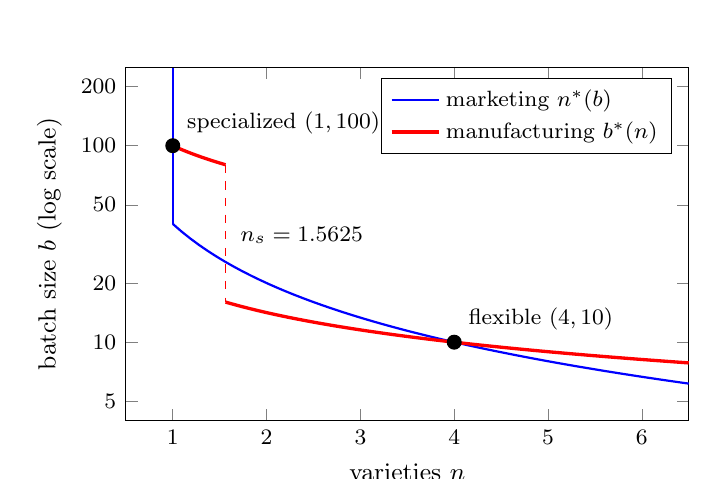
\begin{tikzpicture}
\begin{axis}[
  width=0.72\linewidth, height=0.5\linewidth,
  xmin=0.5, xmax=6.5, ymin=4, ymax=250, ymode=log,
  xlabel={varieties $n$}, ylabel={batch size $b$ (log scale)},
  ytick={5,10,20,50,100,200}, yticklabels={5,10,20,50,100,200},
  xtick={1,2,3,4,5,6},
  legend pos=north east, legend style={font=\footnotesize, cells={anchor=west}},
  tick label style={font=\footnotesize}, label style={font=\small},
  clip=false]
  % marketing: n = max{1, 40/b}
  \addplot[thick, blue, domain=1:6.5, samples=60] {40/x};
  \addlegendentry{marketing $n^*(b)$}
  \addplot[very thick, red, domain=1:1.5625, samples=20] {100/sqrt(x)};
  \addlegendentry{manufacturing $b^*(n)$}
  \addplot[thick, blue, forget plot] coordinates {(1,40) (1,250)};
  \addplot[very thick, red, domain=1.5625:6.5, samples=60, forget plot] {20/sqrt(x)};
  \addplot[red, dashed, forget plot] coordinates {(1.5625,80) (1.5625,16)};
  \node[font=\footnotesize, anchor=west] at (axis cs:1.62,35) {$n_s = 1.5625$};
  \addplot[only marks, mark=*, mark size=2.5pt, black, forget plot]
    coordinates {(1,100) (4,10)};
  \node[font=\footnotesize, anchor=south west] at (axis cs:1.05,102) {specialized $(1,100)$};
  \node[font=\footnotesize, anchor=south west] at (axis cs:4.05,10.3) {flexible $(4,10)$};
\end{axis}
\end{tikzpicture}
\caption{Figure 4.3 made exact, with $A=20$, $Q=100$, $h=1$, $S_s=50$, $S_F=2$, $\Delta c=1$.
Marketing's reply is $n^*(b)=\max\{1,2A/(hb)\}$ (vertical at $n=1$ for $b\ge 40$); manufacturing's
reply $b^*(n)=\sqrt{2SQ/(hn)}$ jumps from 80 to 16 at $n_s=1.5625$, where it switches from
specialized to flexible equipment. The two crossings are the two coherent systems.}
\label{fig:a1-fig43}
\end{figure}

\subsection{What the figure teaches}\label{sec:a1-teaches}

\begin{itemize}
  \item \textbf{Alignment is not optimality.} Each crossing is ``a coherent strategy'' \pg{112};
    ``only one combination is actually profit maximizing'' \pg{112}. Ford's crossing was best for
    the early century; the many-varieties, small-batch crossing is best for many industries now
    \pg{112}.
  \item \textbf{Local adjustment cannot find the global shift.} Managers can track the
    \emph{local} movement of their own crossing, ``but recognizing that a radical strategic shift is
    desirable is likely to require information that neither manager has'' \pg{113}. Smooth changes
    in the curves can hide a jump in which crossing is best \pg{112}.
  \item \textbf{So the choice among coherent patterns is a job for central management} (p.~113,
    p.~115), with innovation attributes, because the information is outside the organization. This
    is Aula 7's argument, met here first.
\end{itemize}

\begin{caution}{A careful reading of footnote 9}
\MR\ picture the profit surface as ``a mountain with three peaks, one at each of the
intersections'' \pg{112}. With two \emph{smooth} decreasing best replies that cross three times,
the middle crossing is a \textbf{saddle}, not a peak: there the replies cross the ``wrong'' way,
$\pi_{nb}^2 > \pi_{nn}\pi_{bb}$, and the Hessian is indefinite. The outer two crossings are the
peaks. The book's point is unaffected: several coherent systems, one best.
\end{caution}

\begin{keyidea}
The companion \texttt{two\_systems.html} (Two Coherent Systems) illustrates this: its plate 1 is
Figure 4.3, its plate 2 the ``ridge line'' of footnote 9, and its presets \emph{More taste for
variety} and \emph{Cheaper flexibility} move each system a little while the best one switches.
\end{keyidea}

% ---------------------------------------------------------------------------------------------
\section{The valley, and the plant that tested it}\label{sec:a1-valley}

\subsection{Three practices on a cube}\label{sec:a1-cube}

Take three Toyota practices from \S\ref{sec:a1-toyota}: just-in-time $J$, multi-skilled teams $T$,
long-term suppliers $S$, each 0 or 1. The class's stylized payoff:
\[
  \pi(J, T, S) = 10 - 4J - 2T - S + 4JT + 5JS + 2TS + 2JTS .
\]

\begin{center}
\small
\setlength{\tabcolsep}{4pt}
\begin{tabular}{@{}lcccccccc@{}}
\toprule
Corner & 000 & 100 & 010 & 001 & 110 & 101 & 011 & 111 \\
\midrule
Profit & \textbf{10} (Ford) & 6 & 8 & 9 & 8 & 10 & 9 & \textbf{16} (Toyota) \\
\bottomrule
\end{tabular}
\end{center}

\begin{itemize}
  \item Supermodular: the pairwise gains $4 + 2S$, $5 + 2T$, $2 + 2J$ are all positive.
  \item \textbf{Every first step loses}: 6, 8, 9 $<$ 10. Ford's corner is a local peak.
  \item \textbf{Every adoption order dips.} Of the six orders from 000 to 111, the best one still
    falls to 9 before reaching 16.
  \item 111 is also a local peak (its neighbours earn 9, 10, 8). Two peaks, and marginal analysis
    cannot tell them apart: the package gain is $+6$; the best single step is $-1$.
\end{itemize}

\begin{figure}[ht]
\centering
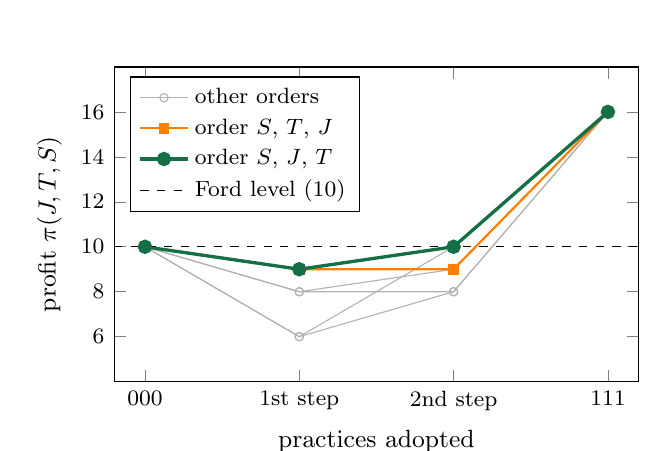
\begin{tikzpicture}
\begin{axis}[
  width=0.68\linewidth, height=0.46\linewidth,
  xmin=-0.2, xmax=3.2, ymin=4, ymax=18,
  xtick={0,1,2,3}, xticklabels={000,1st step,2nd step,111},
  ytick={6,8,10,12,14,16},
  xlabel={practices adopted}, ylabel={profit $\pi(J,T,S)$},
  legend pos=north west, legend style={font=\footnotesize, cells={anchor=west}},
  tick label style={font=\footnotesize}, label style={font=\small}]
  \addplot[gray!60, mark=o, mark size=1.5pt] coordinates {(0,10) (1,6) (2,8) (3,16)};
  \addlegendentry{other orders}
  \addplot[gray!60, mark=o, mark size=1.5pt, forget plot] coordinates {(0,10) (1,6) (2,10) (3,16)};
  \addplot[gray!60, mark=o, mark size=1.5pt, forget plot] coordinates {(0,10) (1,8) (2,8) (3,16)};
  \addplot[gray!60, mark=o, mark size=1.5pt, forget plot] coordinates {(0,10) (1,8) (2,9) (3,16)};
  \addplot[orange, thick, mark=square*, mark size=1.5pt] coordinates {(0,10) (1,9) (2,9) (3,16)};
  \addlegendentry{order $S$, $T$, $J$}
  \addplot[exc, very thick, mark=*, mark size=2pt] coordinates {(0,10) (1,9) (2,10) (3,16)};
  \addlegendentry{order $S$, $J$, $T$}
  \addplot[black, dashed, domain=-0.2:3.2] {10};
  \addlegendentry{Ford level (10)}
\end{axis}
\end{tikzpicture}
\caption{Profit along the six adoption orders from 000 (Ford) to 111 (Toyota), read off the corner
table. Every order dips below the Ford level 10; the best orders, which adopt $S$ first, fall to 9
before reaching 16.}
\label{fig:a1-valley}
\end{figure}

\begin{keyidea}
Complementarity tells you \textbf{where} the optimum is (all practices together). It does not make
the road uphill. It \textbf{creates} the valley, because a practice is worth least where its
complements are missing.
\end{keyidea}

\begin{keyidea}
The companion \texttt{valley.html} (The Valley Between Systems) illustrates this: its preset
\emph{No interactions} shows ``best practices'' thinking (profits add up and the package loses),
and \emph{No stand-alone losses} lets some order climb without a dip.
\end{keyidea}

\subsection{NUMMI: the same workers under two systems}\label{sec:a1-nummi}

History outside \MR\ (sources and status in
\texttt{Videos/\allowbreak aula-01-does-organization-matter/\allowbreak provenance.md}):

\begin{itemize}
  \item GM closed its Fremont, California plant in 1982. It reopened in 1984 as \textbf{NUMMI}, a
    GM--Toyota joint venture run on Toyota's system, and over 85\% of its first workforce were the
    laid-off GM workers.
  \item 1987 assembly hours per car: \textbf{31} at a comparable GM plant (Framingham),
    \textbf{19} at NUMMI, 16 at Toyota's Takaoka plant; assembly defects per 100 cars 135, 45 and
    45. These figures come from a secondary reproduction of Womack, Jones \& Roos (1990) and are
    marked \emph{to confirm against the book}.
  \item GM owned half the plant and its managers could study it, yet its efforts to spread the
    system piece by piece across its US plants ``proved largely unsuccessful''. The exception was
    Brazil, where NUMMI-trained managers ran the transfer.
\end{itemize}

Read with \S\ref{sec:a1-cube}: Toyota moved the whole system at once (the jump across the valley).
GM, adopting practice by practice, kept landing on the low corners.

\subsection{Evidence beyond one plant}\label{sec:a1-evidence}

A test regression: $y = \beta_0 + \beta_1 x + \beta_2 z + \beta_3 x z + \varepsilon$. The effect of
$x$ is $\beta_1$ when $z = 0$ and $\beta_1 + \beta_3$ when $z = 1$: $\beta_3$ is the cross effect.
Ichniowski, Shaw \& Prennushi (1997, \emph{AER} 87(3), 291--313), on 36 steel finishing lines: the
bundle of innovative HR practices raises productivity; single practices adopted in isolation do
not.

\begin{caution}{Correlated adoption is not proof}
Firms that adopt practices together may differ in other ways, so correlated adoption alone does
not prove complementarity.
\end{caution}

% ---------------------------------------------------------------------------------------------
\section{Common mistakes}\label{sec:a1-mistakes}

\begin{center}
\small
\begin{tabularx}{\linewidth}{@{}>{\raggedright\arraybackslash}p{0.33\linewidth}
  >{\raggedright\arraybackslash}X@{}}
\toprule
Mistake & Correction \\
\midrule
``Copy best practices one at a time'' & Profit is not additive; with complements, a practice
  adopted alone can lose money (\S\ref{sec:a1-def}, \S\ref{sec:a1-cube}). \\
``Complements means each is good'' & Complements means each is \emph{better with} the other. Both
  can lose alone (the $2\times2$ table). \\
``A coherent system is the best system'' & Coherence is a local property. Several coherent
  systems coexist; only one is best (\S\ref{sec:a1-teaches}). \\
``If it is better, managers will drift to it'' & Marginal adjustment stays at a local peak;
  reaching the other needs a coordinated jump (pp.~112--113). \\
Using the market definition of complements (cross-price) for internal choices & \MR's definition
  is about marginal profitability, $\partial^2\pi/\partial x_i\partial x_j \ge 0$ \pg{108}. \\
``Substitutes have a multiplier below one'' & In the two-choice model the own response is
  amplified for either sign of $b$; only the other choice's direction changes
  (\S\ref{sec:a1-move}). \\
Reading organization as the org chart & ``not about how berries are arranged on a tree of
  authority but about how people are coordinated and motivated'' \pg{16}. \\
\bottomrule
\end{tabularx}
\end{center}

% ---------------------------------------------------------------------------------------------
\section{Exercises (number and page only)}\label{sec:a1-exercises}

\begin{center}
\small
\begin{tabularx}{\linewidth}{@{}>{\raggedright\arraybackslash}p{0.3\linewidth}
  l >{\raggedright\arraybackslash}X@{}}
\toprule
Exercise & Where & Practises \\
\midrule
\MR\ Food for Thought 1.1 & p.~18 & splitting a business's decisions between centre and units;
  coordination vs.\ motivation \\
\MR\ Food for Thought 1.2 & p.~18 & the same split in a non-business organization \\
\MR\ Food for Thought 1.3 & p.~18 & the Salomon incentive scheme (\S\ref{sec:a1-cases}) against a
  later scandal \\
Cabral 1.1 & p.~11 & competition and performance \\
Cabral 3.14 & p.~63 & sustained competitive advantage (\S3.5) \\
Cabral 3.20 & p.~64 & productivity dispersion across firms (applied, data) \\
\bottomrule
\end{tabularx}
\end{center}

For the formal part (\S\ref{sec:a1-compl}--\S\ref{sec:a1-valley}) there are no book exercises in
\MR\ Ch.~1; use the companions' presets as problems: predict the read-out, then move the control.

% ---------------------------------------------------------------------------------------------
\section*{Sources}
\addcontentsline{toc}{section}{Sources}

\begin{itemize}
  \item Milgrom, P.\ \& Roberts, J.\ (1992). \emph{Economics, Organization, and Management}.
    Prentice-Hall. Ch.~1 (pp.~2--18), Ch.~4 (pp.~106--115). Read from \texttt{Livros/} on
    2026-10-09.
  \item Milgrom, P.\ \& Roberts, J.\ (1990). ``The Economics of Modern Manufacturing: Technology,
    Strategy, and Organization''. \emph{American Economic Review} 80(3), 511--528.
  \item Cabral, L.\ (2017). \emph{Introduction to Industrial Organization}, 2nd ed. MIT Press.
    \S3.5, pp.~56--59.
  \item Ichniowski, C., Shaw, K.\ \& Prennushi, G.\ (1997). \emph{American Economic Review} 87(3),
    291--313.
  \item Ford and NUMMI history: \texttt{Videos/\allowbreak aula-01-does-organization-matter/\allowbreak provenance.md}
    (each claim with its source and status).
\end{itemize}


\newpage
\part{Aula 2 --- Bargaining}
% Part II --- Bargaining (draft Aulas 2-3). Numbers checked by check_part2.py.

\textbf{Read.} \MR{} Ch.~2, ``Wealth Effects, Value Maximization and the Coase Theorem''
(pp.~35--39); Ch.~5, ``Achieving Commitment'' (pp.~133, 139--140), ``Private Information and
Precontractual Opportunism'' and ``Measurement Costs and Investments in Bargaining Position''
(pp.~140--149). Varian (2014, with Calculus) \S30.7 ``Bargaining'' and ``The Ultimatum Game''
(pp.~581--583), \S35.2 (p.~670). MWG Ch.~9, Appendix~A (pp.~296--299). Cabral (2017) \S5.1
(pp.~96--99).

In the draft schedule, Bargaining takes two classes: Aula~2 covers
\S\ref{sec:b-question}--\S\ref{sec:b-nash} (value maximization, Coase, the division of the
gains), and Aula~3 covers \S\ref{sec:b-rub}--\S\ref{sec:b-costs} (alternating offers,
commitment, private information, bargaining costs).

% ---------------------------------------------------------------------------------------
\section{The question: is bargaining indeterminate?}\label{sec:b-question}

Every organization runs on agreements: a supplier contract, a division of profits among
partners, a transfer price between divisions, a wage. Each agreement is reached by some form of
bargaining. \MR{} open the topic with the traditional view that ``the outcomes of bargaining among
small numbers of people are essentially indeterminate'': bargaining strength, credibility,
guile, patience and strategic insight combine with initial conditions to decide the outcome,
and predicting it ``was too much for economic analysis'' \pg{140}.

This Part gives \MR's answer in three steps.

\begin{enumerate}
  \item \textbf{What is created is determinate.} When preferences show no wealth effects, every
  efficient agreement chooses the actions that maximize the parties' total value (the
  \emph{value maximization principle}). Bargaining power decides only the money transfers (the
  \emph{Coase theorem}). Sections~\ref{sec:b-wealth}--\ref{sec:b-coase}.
  \item \textbf{Who gets what can be modelled.} The Nash solution and the Rubinstein
  alternating-offers game turn ``bargaining power'' into threat points, patience and the right
  to propose. Under complete information these models predict immediate, efficient agreement.
  Sections~\ref{sec:b-nash}--\ref{sec:b-commit}.
  \item \textbf{Private information and bargaining costs break efficiency.} When each side knows
  something the other does not, the full-information efficient outcome can be infeasible, and
  even the best feasible arrangement gives up some gains. Time, haggling and information spent
  on shifting the division are wasted. Sections~\ref{sec:b-private}--\ref{sec:b-costs}.
\end{enumerate}

Throughout, a decision has two parts: $y$, the \emph{real} choice (what is produced, who owns
an asset, whether a project is built), and $x = (x_1,\dots,x_N)$, the money transfers among the
parties.

% ---------------------------------------------------------------------------------------
\section{Wealth effects and the value index}\label{sec:b-wealth}

A \emph{wealth effect} is a change in choices caused by a change in wealth: a poorer person may
be unable to afford an option, or may trade off risk differently \pg{35}.

\begin{defn}{No wealth effects \pg{35}}
A decision maker shows \emph{no wealth effects} with respect to a set of decisions $Y$ when, for
any two decisions $y_1, y_2 \in Y$:
\begin{enumerate}[label=(\roman*)]
  \item there is a definite amount of money $\Delta x$ that would just compensate him or her for
  a switch from $y_1$ to $y_2$;
  \item that amount does not change if he or she is first given extra wealth;
  \item he or she has enough money to absorb any wealth reduction needed to pay for a switch
  from the less preferred to the more preferred option.
\end{enumerate}
\end{defn}

\begin{prop}{Proposition 1 (the value index, \MR{} p.~36 and n.~7)}
Under no wealth effects, preferences over (money $x$, decision $y$) can be represented by
\[
  u(x, y) = x + v(y),
\]
where $v(y)$ is the cash-equivalent value of $y$. The compensating transfer for a switch from
$y_1$ to $y_2$ is $\Delta x = v(y_1) - v(y_2)$, the same at every initial wealth $M$.
\end{prop}

\emph{Why.} With $u = x + v(y)$, the person is indifferent between $(M, y_1)$ and
$(M + \Delta x, y_2)$ exactly when $M + v(y_1) = M + \Delta x + v(y_2)$, so
$\Delta x = v(y_1) - v(y_2)$: it exists (condition i) and does not depend on $M$ (condition ii).
Condition (iii) holds as long as $M$ exceeds the largest difference $|v(y) - v(y')|$. Conversely,
\MR's Q~2.4 (p.~53) asks you to show that conditions like (i)--(ii) force this form.

\textbf{Where it fails.} \MR{} contrast two cases \pg{35--36}. A corporation that finds itself
richer after a rise in its asset values would plausibly keep the same prices and hurdle rates:
no wealth effects. A worker who wins the lottery buys a house and quits: large wealth effects.
Condition (iii) fails when the transfer is large relative to the person's resources, as with a
nuclear-plant worker made financially liable for his or her mistakes \pg{36}. The rule of thumb:
the assumption is least safe ``when the decision makers are individuals and when large cash
transfers or significant changes in personal living conditions are involved'' \pg{36}.

\begin{example}{With wealth effects, who holds the right changes what is done}
A plant gains $50$ (in money) from dumping waste in a river. A resident with wealth $w = 100$ has
utility $u = \ln x + a\,y$, where $y = 1$ if the river is clean and $a = 0.5$. This is not of
the form $x + v(y)$: the money value of a clean river depends on wealth.

\emph{Willingness to pay} for a clean river (resident owns nothing, must buy it):
$\ln(w - P) + a = \ln w \;\Rightarrow\; P = w(1 - e^{-a}) \approx 39.35$.

\emph{Willingness to accept} for giving the river up (resident owns the right):
$\ln(w + A) = \ln w + a \;\Rightarrow\; A = w(e^{a} - 1) \approx 64.87$.

If the plant holds the right, the resident can offer at most $39.35 < 50$: the plant dumps. If
the resident holds it, the plant would have to pay at least $64.87 > 50$: the river stays
clean. The \emph{real} outcome $y$ depends on the assignment of rights. With wealth effects, the
gap between willingness to pay and to accept makes ``the efficient choice'' depend on who starts
with what, and the clean separation of the next section disappears.
\end{example}

% ---------------------------------------------------------------------------------------
\section{The value maximization principle}\label{sec:b-vmp}

\begin{prop}{The Value Maximization Principle (\MR{} p.~36)}
``An allocation among a group of people whose preferences display no wealth effects is efficient
only if it maximizes the total value of the affected parties. Moreover, for any inefficient
allocation, there exists another (total value maximizing) allocation that all of the parties
strictly prefer.''
\end{prop}

\textbf{Setting.} $N$ people with $u_n(x_n, y) = x_n + v_n(y)$. Decision $y$ generates net cash
$P(y)$ (positive for an investment, negative for a public good that costs money), and the
transfers must add up: $x_1 + \dots + x_N = P(y)$. The \emph{total value} of an allocation is
\[
  \sum_{n} \big[x_n + v_n(y)\big] \;=\; P(y) + \sum_n v_n(y) \;\equiv\; W(y),
\]
which depends on $y$ alone: changing the $x$'s moves value between people one for one and never
changes the total.

\begin{prop}{Proposition 2 (efficiency $\Leftrightarrow$ value maximization)}
An allocation $(y, x_1, \dots, x_N)$ is Pareto efficient if and only if $y \in \argmax_{y'} W(y')$.
\end{prop}

\begin{proof}
($\Leftarrow$) Let $y$ maximize $W$ and suppose another allocation $(y', x')$ made everyone at
least as well off and someone strictly better off. Summing utilities,
$W(y') = \sum_n [x'_n + v_n(y')] > \sum_n [x_n + v_n(y)] = W(y)$, contradicting the maximality of
$W(y)$.

($\Rightarrow$) Suppose $y$ does not maximize $W$: some $y^*$ has $G \equiv W(y^*) - W(y) > 0$.
Give each person the transfer
\[
  x^*_n = x_n + v_n(y) - v_n(y^*) + \frac{G}{N}.
\]
Then $u_n(x^*_n, y^*) = x_n + v_n(y) + G/N > u_n(x_n, y)$ for every $n$. The transfers add up:
using $\sum_n x_n = P(y)$ and $G = P(y^*) + \sum_n v_n(y^*) - P(y) - \sum_n v_n(y)$,
\[
  \sum_n x^*_n = P(y) + \sum_n v_n(y) - \sum_n v_n(y^*) + G = P(y^*).
\]
So every inefficient allocation is strictly Pareto dominated by a value-maximizing one, which is
the second sentence of the principle.
\end{proof}

\MR's Q~2.3 (p.~53) asks for this proof; the hint there is the equal-split construction used
above. The proof uses condition (iii): the transfers $x^*_n$ must be affordable.

\begin{figure}[ht]
\centering
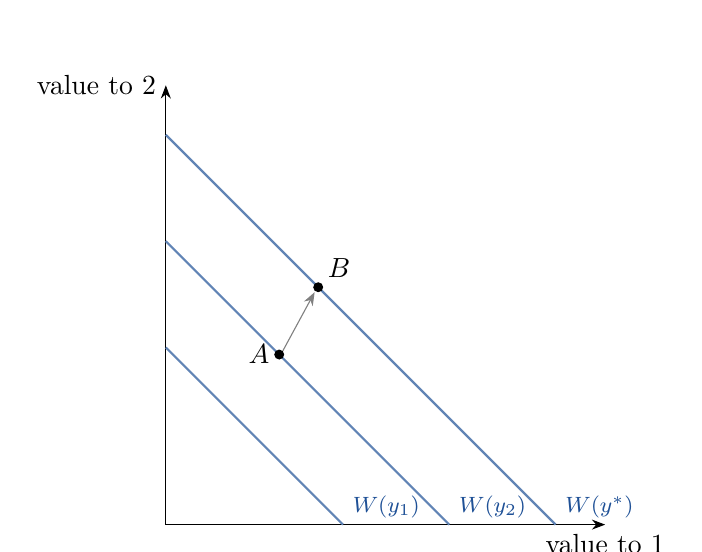
\begin{tikzpicture}[scale=0.9,>=Stealth]
  \draw[->] (0,0) -- (6.2,0) node[below] {value to 1};
  \draw[->] (0,0) -- (0,6.2) node[left] {value to 2};
  \foreach \c/\lab in {2.5/{$W(y_1)$}, 4/{$W(y_2)$}, 5.5/{$W(y^*)$}} {
    \draw[thick, defc!70] (0,\c) -- (\c,0);
    \node[defc, font=\footnotesize, right] at (\c,0.25) {\lab};
  }
  \fill (1.6,2.4) circle (2pt) node[left] {$A$};
  \fill (2.15,3.35) circle (2pt) node[above right] {$B$};
  \draw[->, gray] (1.65,2.45) -- (2.1,3.28);
\end{tikzpicture}
\caption{\MR's Figure 2.1 (p.~37). Each line is the set of value pairs reachable with one
decision $y$ as the transfers vary; lines are at $45^\circ$ because transfers move value one for
one. Any point $A$ on a lower line is dominated by some $B$ on the highest line; points on the
highest line are undominated.}
\end{figure}

\begin{keyidea}
When the principle applies, ``the issue of the distribution of value is completely separable
from the issue of how value is created'' \pg{38}. Efficiency picks $y$; everything else
(bargaining power, patience, initial ownership) only moves the $x$'s.
\end{keyidea}

\textbf{The limit (\MR{} n.~10, p.~37).} With wealth effects, an allocation that maximizes the
sum of utilities is still efficient, but there can be efficient allocations that do not: value
maximization becomes \emph{sufficient} but not \emph{necessary} for efficiency. The utility
possibility frontier is then curved rather than a $45^\circ$ line, and different points on it
can use different $y$'s (as in the river example above).

\textbf{Range of application} \pg{38}. The variable $y$ can be the money spent on parks or
libraries, the identity of the person assigned overtime, the owner of water rights, the brand of
computer adopted, or the site of a new office building. In each case the principle says the
group should, and if it bargains efficiently will, pick the $y$ with the largest total value,
then settle shares by transfers.

% ---------------------------------------------------------------------------------------
\section{The Coase theorem}\label{sec:b-coase}

\begin{prop}{The Coase Theorem (\MR{} p.~38)}
``If the parties bargain to an efficient agreement (for themselves) and if their preferences
display no wealth effects, then the value-creating activities ($y$) that they will agree upon do
not depend on the bargaining power of the parties or on what assets each owned when the
bargaining began. Rather, efficiency alone determines the activity choice. The other factors can
affect only decisions about how the costs and benefits are to be shared ($x$).''
\end{prop}

The theorem is the value maximization principle plus one behavioural assumption: the parties
reach an agreement with no further mutual gains. Its organizational corollary is \MR's
foundation for the transaction-costs approach: for a given production plan, ``the efficient
organization for that plan is the one that minimizes transaction costs'' \pg{38}, where
transaction costs include writing contracts, supervising, enforcing and resolving disputes.

\begin{example}{The steel plant and the river (after Cabral, pp.~97--98)}
Cabral's setting: a steel plant can dump waste in a river, harming residents downstream; society
can give the right to clean water to the residents or the right to dump to the plant. Put
numbers on it: dumping is worth $100$ to the plant and costs the residents $60$, everyone has
no wealth effects, and bargaining is costless.

\begin{itemize}
  \item \emph{Plant holds the right.} The residents would pay at most $60$ to stop dumping; the
  plant needs at least $100$. No deal: the plant dumps, no money changes hands.
  \item \emph{Residents hold the right.} The plant can pay anything in $[60, 100]$ for
  permission. With an even split of the $40$ gain (the Nash solution of \S\ref{sec:b-nash}),
  the price is $60 + 20 = 80$. The plant dumps.
\end{itemize}
Dumping happens either way, because it creates $100 - 60 = 40$ of value. The assignment of rights
only decides whether residents end up $80 - 60 = +20$ or $0$, and the plant $+20$ or $+100$.
Reverse the numbers (harm $100$, gain $60$) and the river stays clean under either assignment.
\end{example}

Cabral draws the lesson that the Coase theorem is about efficiency, not fairness: ``From an
efficiency point of view, it makes no difference who owns the rights to a clean river (factory or
residents). This is not to say, however, that both property rights allocations are equally
fair'' (Cabral, p.~99). Varian's \S35.2 makes the same point in consumer theory: with
quasilinear preferences the efficient amount of the externality is independent of the
assignment of property rights, and only the distribution changes (Varian, p.~670).

\textbf{When the theorem fails.} Each hypothesis can break:
\begin{enumerate}
  \item \emph{Wealth effects and limited capital.} The implications ``do not hold when some of the
  parties have very limited capital with which to make payments''. \MR{} would apply the analysis
  to a contract between General Motors and Toyota, but not ``uncritically'' to land tenure in a
  developing country or to slavery in the pre-Civil War American South \pg{39}.
  \item \emph{Costly bargaining.} Haggling, delay and measurement absorb part of the gains
  (\S\ref{sec:b-costs}).
  \item \emph{Private information.} Efficient bargaining is an assumption of the theorem, not a
  result: with private values, no feasible procedure may reach the efficient $y$
  (\S\ref{sec:b-private}).
  \item \emph{Many parties.} Free riding makes unanimous agreement harder as the group grows
  (\S\ref{sec:b-many}).
\end{enumerate}

\textbf{Rival explanations of organization} \pg{39}. The transaction-costs view says
arrangements exist to raise the total wealth to be shared. Against the \emph{Marxian} view
(organization reflects power and class interests), \MR{} cite Yugoslavia, where worker-controlled
firms hired managers who organized factories much like capitalist firms. Against the
\emph{Harvard school} of industrial organization (arrangements raise market power), they read
resale price maintenance as a defence against discounters free riding on the service and customer
education provided by other dealers. They add that only systematic evidence can decide between
the views.

\begin{caution}{Three misreadings of Coase}
(1) ``Property rights do not matter.'' They matter for the distribution, and with wealth effects
for the allocation too. (2) ``Externalities are never a problem.'' The theorem assumes efficient,
costless bargaining; its practical lesson is to look for the transaction costs that block it.
(3) ``Coase predicts a fair outcome.'' It predicts an efficient $y$ and says nothing about $x$.
\end{caution}

% ---------------------------------------------------------------------------------------
\section{Dividing the gains: the Nash bargaining solution}\label{sec:b-nash}

The value maximization principle leaves the transfers open. Two families of models close them.
The \emph{axiomatic} approach asks which division satisfies reasonable properties; the
\emph{strategic} approach (next section) writes down the bargaining procedure as a game. Varian
introduces both and notes that the outcome of the Nash model depends ``on how risk averse the
players are and what will happen if no bargain is made'', leaving its full treatment out of his
book (Varian, p.~581). The statement below is the standard one (Nash 1950), not taken from the
course books.

\begin{defn}{Bargaining problem and Nash solution}
Two players can agree on a pair of payoffs $(u_1, u_2)$ in a feasible set $U$, or fail to agree
and get the \emph{threat point} (disagreement point) $d = (d_1, d_2)$. The Nash bargaining
solution is the unique rule satisfying Pareto efficiency, symmetry, invariance to affine
rescaling of utilities and independence of irrelevant alternatives; it selects
\[
  (u_1^N, u_2^N) \in \argmax_{(u_1, u_2) \in U,\; u_i \ge d_i} \; (u_1 - d_1)(u_2 - d_2).
\]
\end{defn}

With no wealth effects the frontier is the $45^\circ$ line $u_1 + u_2 = V$, where
$V = \max_y W(y)$ is the maximal total value. Maximizing $(u_1 - d_1)(V - u_1 - d_2)$ gives
\[
  u_1^N = d_1 + \tfrac{1}{2}\,(V - d_1 - d_2), \qquad u_2^N = d_2 + \tfrac{1}{2}\,(V - d_1 - d_2):
\]
each party gets its threat point plus half the \emph{surplus} $V - d_1 - d_2$. The
\emph{generalized} Nash solution maximizes $(u_1 - d_1)^{\alpha}(u_2 - d_2)^{1-\alpha}$ and gives
party~1 the share $\alpha$ of the surplus: $u_1 = d_1 + \alpha(V - d_1 - d_2)$.

\begin{keyidea}
Threat points and bargaining weights move the transfers, never the real decision: every
solution sits on the line $u_1 + u_2 = V$, so it uses a value-maximizing $y$. To get a larger
share, improve your outside option ($d_i$) or your bargaining weight ($\alpha$), not the size
of $V$. Section~\ref{sec:b-costs} shows why that private incentive is socially wasteful.
\end{keyidea}

% ---------------------------------------------------------------------------------------
\section{Alternating offers}\label{sec:b-rub}

\subsection{Finite horizon (MWG Example 9.AA.1; Stahl 1972)}

Two players divide $v$ dollars. In odd periods player~1 offers a split and player~2 accepts or
rejects; in even periods the roles swap. A dollar received in period $t$ is worth $\delta^{t-1}$
today, $\delta \in (0,1)$. If no agreement is reached by period $T$, both get nothing
(MWG, p.~296).

\begin{prop}{Proposition 3 (finite horizon)}
The game has a unique subgame perfect Nash equilibrium (SPNE). Agreement is reached at once, and
the first proposer receives
\[
  v_1(T) = v\,\big[1 - \delta + \delta^2 - \dots + (-\delta)^{T-1}\big]
         = v\,\frac{1 - (-\delta)^{T}}{1 + \delta},
\]
which is $v\,(1 + \delta^T)/(1+\delta)$ for odd $T$ and $v\,(1 - \delta^T)/(1+\delta)$ for even $T$.
Player~2 receives $v - v_1(T)$.
\end{prop}

\begin{proof}
Backward induction. In period $T$ the responder accepts any offer (rejecting gives zero), so the
proposer takes everything: share $s_1 = 1$. In period $T-1$ the responder is the next proposer;
rejecting is worth $\delta \cdot s_1$ to him or her in period-$(T-1)$ terms, so the proposer
offers exactly that and keeps $s_2 = 1 - \delta s_1$. In general $s_{k+1} = 1 - \delta s_k$ with
$s_1 = 1$, whose solution is $s_k = \sum_{j=0}^{k-1}(-\delta)^j$. At $k = T$ this is the formula.
Uniqueness: in each subgame the responder accepts iff the offer is at least the continuation
value (accepting at indifference, as MWG and Varian assume), and the proposer's best offer is
pinned down.
\end{proof}

Two lessons. \emph{Who proposes last matters}: with $T = 1$ the proposer takes everything; with
$T = 2$ the second mover gets $\delta v$. \emph{The horizon matters less and less}: as
$T \to \infty$, $v_1(T) \to v/(1+\delta)$ whichever player moves last. With $\delta = 0.6$:
$v_1(3) = 1 - 0.6 + 0.36 = 0.76$, and $v_1(T) \to 0.625$.

\begin{example}{Varian's three-day game (Varian, pp.~581--582)}
Alice and Bob divide \$1 over at most three days; Alice offers on days 1 and 3, Bob on day 2.
Alice discounts at $\alpha$ per day, Bob at $\beta$. On day 3 Alice takes everything. On day 2,
Bob must offer Alice $\alpha$ (the value of \$1 tomorrow) and keeps $1 - \alpha$. On day 1, Alice
must offer Bob $\beta(1 - \alpha)$ and keeps
\[
  1 - \beta(1 - \alpha).
\]
Each party's share rises with its \emph{own} patience: a patient Alice ($\alpha$ near 1) leaves
Bob little to protect on day 2.
\end{example}

\subsection{Infinite horizon: Rubinstein (MWG Example 9.AA.2)}

Remove the deadline and let the players' discount factors differ, $\delta_1, \delta_2 \in (0,1)$.

\begin{prop}{Proposition 4 (Rubinstein 1982)}
The infinite-horizon alternating-offers game has a unique SPNE. Player~1 offers at once
\[
  x_1^* = \frac{1 - \delta_2}{1 - \delta_1\delta_2}, \qquad x_2^* = \frac{\delta_2(1 - \delta_1)}{1 - \delta_1\delta_2},
\]
and player~2 accepts. With $\delta_1 = \delta_2 = \delta$, the shares are $1/(1+\delta)$ and
$\delta/(1+\delta)$, the limit of Proposition~3. In Varian's notation (Alice $\alpha$, Bob
$\beta$): Alice $(1-\beta)/(1-\alpha\beta)$, Bob $\beta(1-\alpha)/(1-\alpha\beta)$ (Varian, p.~582).
\end{prop}

\begin{proof}[Proof sketch (Shaked and Sutton's bounding argument, used by MWG)]
Let $M_1$ and $m_1$ be the supremum and infimum of player~1's SPNE payoffs in any subgame where
he or she proposes, and $M_2, m_2$ the same for player~2 when proposing. The game looks the same
from every proposing node, so these bounds are stationary.
\begin{itemize}
  \item Player~2 rejects anything below $\delta_2 m_2$ and accepts anything above $\delta_2 M_2$.
  So player~1 gets at least $1 - \delta_2 M_2$ and at most $1 - \delta_2 m_2$ (delay only shrinks
  the pie): $m_1 \ge 1 - \delta_2 M_2$ and $M_1 \le 1 - \delta_2 m_2$.
  \item Symmetrically, $m_2 \ge 1 - \delta_1 M_1$ and $M_2 \le 1 - \delta_1 m_1$.
\end{itemize}
Combine: $M_1 \le 1 - \delta_2(1 - \delta_1 M_1)$, so $M_1 \le (1-\delta_2)/(1-\delta_1\delta_2)$;
and $m_1 \ge 1 - \delta_2(1 - \delta_1 m_1)$, so $m_1 \ge (1-\delta_2)/(1-\delta_1\delta_2)$. Hence
$M_1 = m_1 = x_1^*$, and likewise for player~2. The strategies ``always offer the other
$\delta_j x_j^*$, accept any offer of at least $\delta_i x_i^*$'' attain it, and immediate acceptance
follows because any delay loses value both players could share.
\end{proof}

\begin{figure}[ht]
\centering
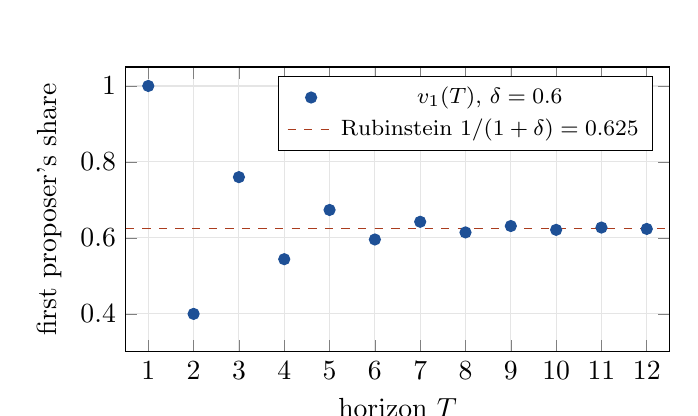
\begin{tikzpicture}
\begin{axis}[width=0.7\linewidth, height=5.2cm, xlabel={horizon $T$},
  ylabel={first proposer's share}, ymin=0.3, ymax=1.05, xmin=0.5, xmax=12.5,
  xtick={1,...,12}, grid=major, grid style={gray!20}, legend pos=north east,
  legend style={font=\footnotesize}]
\addplot[only marks, mark=*, defc] coordinates {(1,1) (2,0.4) (3,0.76) (4,0.544) (5,0.6736)
  (6,0.59584) (7,0.642496) (8,0.6145024) (9,0.63129856) (10,0.621220864) (11,0.627267482)
  (12,0.623639511)};
\addlegendentry{$v_1(T)$, $\delta = 0.6$}
\addplot[dashed, warnc, domain=0.5:12.5] {0.625};
\addlegendentry{Rubinstein $1/(1+\delta) = 0.625$}
\end{axis}
\end{tikzpicture}
\caption{Finite-horizon shares oscillate (the last proposer gains) and converge to the
infinite-horizon share.}
\end{figure}

\textbf{What the model says about bargaining power.}
\begin{enumerate}
  \item \emph{Agreement is immediate and efficient.} Under complete information no value is lost
  to delay: the threat of delay is what divides the surplus, but it is never carried out.
  \item \emph{Patience is power.} $x_1^*$ rises in $\delta_1$ and falls in $\delta_2$. If
  $\delta_1 \to 1$ with $\delta_2 < 1$, player~1 takes everything (Varian, p.~582).
  \item \emph{The first-mover advantage vanishes as offers speed up.} Write
  $\delta_i = e^{-r_i \Delta}$, with $\Delta$ the time between offers. As $\Delta \to 0$,
  $x_1^* \to r_2/(r_1 + r_2)$: the division depends only on relative impatience. With equal
  rates it tends to $1/2$, the symmetric Nash split, which links the strategic model to the
  axiomatic one of \S\ref{sec:b-nash} (Binmore, Rubinstein and Wolinsky 1986; not in the course
  books).
  \item \emph{The real decision is untouched.} Discount factors move $x$, never $y$: the
  alternating-offers game is a model of the transfers in the Coase theorem.
\end{enumerate}

\textbf{Computing it.} The finite-horizon recursion is three lines of Python; it reproduces the
figure and, with $T$ large, Proposition~4 (\texttt{check\_part2.py} uses it):
\begin{verbatim}
def proposer_share(T, d1, d2):    # pie 1; player 1 proposes first
    share = 1.0                   # the last proposer takes everything
    who = (T - 1) % 2             # last proposer: 0 = player 1, 1 = player 2
    for _ in range(T - 1):        # one period back: the responder (who)
        d = d1 if who == 0 else d2   # must get the discounted value of
        share = 1 - d * share        # proposing next period
        who = 1 - who
    return share
\end{verbatim}

% ---------------------------------------------------------------------------------------
\section{Commitment, reputation and the ultimatum game}\label{sec:b-commit}

In alternating offers, power comes from what a player can credibly do next. \emph{Commitment}
changes that by removing options. \MR's examples \pg{133}: in 1066 William the Conqueror burned
his fleet behind his army, and Cort\'es repeated the stratagem in Mexico; the commitment ``deterred
the opposition, who then themselves retreated''. When Apple built a highly specialized plant for
the Macintosh, it made dropping the product more expensive, and so committed itself in the eyes
of employees, competitors and customers. The cost is real: noncontractual commitment ``may be
worthwhile, but costly'': the fleets were perfectly good, and the specialized plant may become
obsolete sooner \pg{139}.

\textbf{Reputation as a substitute} \pg{139--140}. Concern for reputation checks opportunism when
contracts cannot. Its value grows with the frequency of similar transactions, the horizon over
which they recur, and their profitability. Hence, in relational contracts, discretion over
unforeseen events should go to the party with the most to lose from a damaged reputation: the
one with the longer horizon, more visibility, greater size and more frequent transactions,
which in employment is usually the firm, not the employee \pg{140}. Bargaining with terrorists
or renegotiating executive pay advertises that there is no commitment \pg{139}.

\textbf{The ultimatum game} (Varian, pp.~582--583). Alice proposes a division of \$1; if Bob
accepts it is implemented, otherwise both get nothing. The SPNE gives Alice almost everything
(``something like 99 cents''). In experiments, the average offer by U.S. undergraduates is about
45 cents and is usually accepted. Proposers are close to maximizing expected payoff given the
observed rejection rates; it is the responders who depart from the theory, rejecting small offers
at a cost to themselves. Explanations: social norms of fair division, which differ across
cultures, and a taste for punishing unfair offers.

\begin{keyidea}
A one-shot offer is commitment in its purest form: the proposer is committed to walking away.
A responder who could credibly commit to rejecting anything below $k$ would receive $k$. A
known taste for fairness or vengeance acts as exactly such a commitment, which is the question
\MR{} pose in FFT~5.1 (pp.~163--164); FFT~5.2 (p.~164) asks what makes a signal of intent
credible.
\end{keyidea}

% ---------------------------------------------------------------------------------------
\section{Private information: when efficient trade is infeasible}\label{sec:b-private}

\MR's turn is one sentence: efficiency is defined relative to the feasible outcomes, and
``what is feasible---and thus what is efficient---turns out to depend crucially on the
informational conditions'' \pg{140}. With private information, an agreement may not be reached
even when it would be efficient, and if it is reached it is not typically efficient by
full-information standards, ``especially when the parties have an option not to participate''
\pg{140}.

\subsection{\MR's example: bargaining over a sale}

A seller owns one unit; a buyer wants it. Each knows only his or her own value \pg{140--141}:

\begin{center}
\begin{tabular}{lcc}
\toprule
 & Seller's value \$0 (prob.\ 0.8) & Seller's value \$2 (prob.\ 0.2) \\
\midrule
Buyer's value \$1 (prob.\ 0.2) & Trade & No trade \\
Buyer's value \$3 (prob.\ 0.8) & Trade & Trade \\
\bottomrule
\end{tabular}

\smallskip
{\footnotesize Efficient outcomes (\MR{} Table 5.2, p.~141). Trade is efficient with probability
$1 - 0.2 \times 0.2 = 0.96$.}
\end{center}

\textbf{The temptation.} A buyer worth \$3 would like to claim \$1 to pay less; a seller worth
\$0 would like to claim \$2 to be paid more. Misrepresentation risks the sale falling through,
but ``this may be a risk worth taking'' \pg{141}.

\textbf{The mediator device.} Ask whether a neutral mediator who sets prices as a function of the
two reports could make honest reporting optimal \emph{and} trade happen exactly when efficient.
If no mediator can, the parties cannot do it by themselves either \pg{141}. Two kinds of
constraints bind:
\begin{itemize}
  \item \emph{participation constraints}: nobody can be forced to trade at a loss given the
  value he or she reports;
  \item \emph{incentive compatibility constraints}: each type must do at least as well reporting
  truthfully as reporting the other type.
\end{itemize}
The surplus a type must be left to report honestly is its \emph{informational rent} (n.~7, p.~141).

\textbf{Pinning down the prices} (\MR{} Table 5.3, p.~142). A seller who claims \$2 must get at
least \$2, and paying more only rewards the claim: price \$2. A buyer who claims \$1 must pay at
most \$1: price \$1. One price is left, $p$, for reports (seller \$0, buyer \$3).

\begin{center}
\begin{tabular}{lcc}
\toprule
 & Buyer reports \$1 & Buyer reports \$3 \\
\midrule
Seller reports \$0 & price \$1 & price $p$ \\
Seller reports \$2 & no trade & price \$2 \\
\bottomrule
\end{tabular}
\end{center}

\emph{Seller worth \$0} (the buyer reports honestly):
\[
  \underbrace{0.2 \times 1 + 0.8\,p}_{\text{honest}} \;\ge\;
  \underbrace{0.2 \times 0 + 0.8 \times 2}_{\text{claim \$2}} = 1.60
  \quad\Longrightarrow\quad p \ge 1.75 .
\]
\emph{Buyer worth \$3}:
\[
  \underbrace{0.2 \times (3 - 2) + 0.8\,(3 - p)}_{\text{honest}} = 2.60 - 0.8\,p \;\ge\;
  \underbrace{0.8 \times (3 - 1)}_{\text{claim \$1}} = 1.60
  \quad\Longrightarrow\quad p \le 1.25 .
\]
No $p$ satisfies both. ``It is impossible to find any prices that always make it in the parties'
individual interests to report truthfully and to trade whenever trade is, in fact, value
increasing'' \pg{142}.

\begin{defn}{The revelation principle (\MR{} n.~8, pp.~142--143)}
Any pattern of outcomes achievable by any mechanism that respects incentive constraints can be
achieved by a mechanism in which the parties report their values and are given incentives to
report honestly. Hence restricting attention to honest reporting, as above, loses no generality:
the impossibility holds for every bargaining procedure.
\end{defn}

\textbf{Reverse the probabilities} \pg{143}. Let the buyer be worth \$1 with probability 0.8 and
the seller \$2 with probability 0.8, and set $p = 1.50$. A seller worth \$0 gets
$0.8 \times 1 + 0.2 \times 1.50 = 1.10$ by reporting honestly and $0.2 \times 2 = 0.40$ by
claiming \$2. A buyer worth \$3 gets $0.8 \times 1 + 0.2 \times 1.50 = 1.10$ honestly and
$0.2 \times 2 = 0.40$ by claiming \$1. Both constraints hold (checking the low types and participation
too, any $p$ between 0 and 3 works), so efficient trade is attainable.

\begin{keyidea}
Lying about your value is cheap when trade is likely to happen anyway, and expensive when it puts
a likely trade at risk. In the original example the high-value buyer and the low-value seller
each face a partner who is probably willing to trade (probability 0.8), so exaggerating costs
little. Reverse the odds and every misreport kills a trade 80\% of the time \pg{143}.
\end{keyidea}

The example is a discrete instance of a general result for bilateral trade with independent
private values whose supports overlap: no mechanism is efficient, incentive compatible, individually
rational and budget balanced (Myerson and Satterthwaite 1983; the name is not in the course
books).

% ---------------------------------------------------------------------------------------
\section{Incentive efficiency}\label{sec:b-ie}

If incentive constraints cannot be escaped, failing the full-information benchmark is not a
failure of the parties. \MR{} change the benchmark \pg{143}:

\begin{defn}{Incentive efficiency}
A mechanism is \emph{incentive efficient} if no alternative mechanism that is feasible in the
presence of the incentive constraints is preferred by all the relevant parties. By the efficiency
principle, bargainers should be expected to find incentive-efficient mechanisms.
\end{defn}

\subsection{Split-the-difference bargaining}

The buyer's value $B$ and the seller's value $S$ are independent and uniform on $[0,1]$, each
private. Both name a price at once; if the seller's ask $s$ is below the buyer's bid $b$, they
trade at $(s + b)/2$; otherwise both walk away \pg{143}.

\textbf{Small lies pay} \pg{144}. Let the buyer bid truthfully and a seller with $S = 0.50$ ask
$0.52$. Trades are lost only when $B \in (0.50, 0.52)$, probability $0.02$, each losing at most
$\$0.01$ and $\$0.005$ on average: expected loss $0.02 \times 0.005 = \$0.0001$. Against that, the
price rises by $\$0.01$ whenever $B \ge 0.52$ (probability $0.48$): gain $\$0.0048$. Net gain
$\$0.0047$. The losses from misreporting fall on trades that ``were hardly profitable anyway''.

\begin{prop}{Proposition 5 (the linear equilibrium, \MR{} n.~9, p.~144)}
There is an equilibrium in linear strategies
\[
  s(S) = \tfrac14 + \tfrac23 S, \qquad b(B) = \tfrac1{12} + \tfrac23 B,
\]
and trade occurs if and only if $B > S + \tfrac14$.
\end{prop}

\begin{proof}
Suppose the buyer bids $b = \beta_1 + \beta_2 B$. A seller with value $S$ who asks $s$ trades when
$B \ge (s - \beta_1)/\beta_2$ and earns
\[
  \pi_S(s) = \int_{(s-\beta_1)/\beta_2}^{1} \Big(\frac{s + \beta_1 + \beta_2 B}{2} - S\Big)\, dB .
\]
Differentiating (Leibniz rule; at the lower limit the price equals $s$):
$\pi'_S(s) = \tfrac12\big(1 - \tfrac{s - \beta_1}{\beta_2}\big) - \tfrac{1}{\beta_2}(s - S) = 0$,
so $s = \tfrac23 S + \tfrac{\beta_1 + \beta_2}{3}$. Symmetrically, if the seller asks
$\sigma_1 + \sigma_2 S$, a buyer with value $B$ who bids $b$ trades when $S \le (b - \sigma_1)/\sigma_2$
and the first-order condition gives $b = \tfrac23 B + \tfrac{\sigma_1}{3}$. Matching
coefficients: $\sigma_2 = \beta_2 = \tfrac23$, $\sigma_1 = (\beta_1 + \tfrac23)/3$,
$\beta_1 = \sigma_1/3$, so $\sigma_1 = \tfrac14$ and $\beta_1 = \tfrac1{12}$. Finally
$b > s \iff \tfrac1{12} + \tfrac23 B > \tfrac14 + \tfrac23 S \iff B > S + \tfrac14$.
\end{proof}

\textbf{How much is lost.} Let $D = B - S$; on $[0,1]$ its density is $1 - D$. Efficient trade
happens with probability $\tfrac12$ and creates expected gains $\int_0^1 D(1-D)\,dD = \tfrac16$.
In equilibrium trade happens with probability $\int_{1/4}^{1}(1 - D)\,dD = \tfrac{9}{32}$, and the
realized gains are $\int_{1/4}^{1} D(1-D)\,dD = \tfrac{9}{64}$, which is $\tfrac{27}{32} \approx 84\%$
of the efficient total. Trade is cut almost in half, but surplus by only 16\%, because the trades
lost are the ones with small gains.

\begin{figure}[ht]
\centering
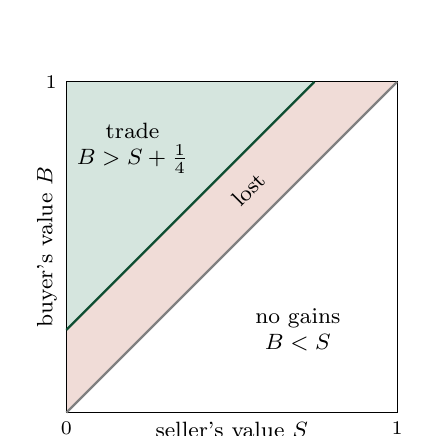
\begin{tikzpicture}[scale=4.2]
  \fill[exc!18] (0,0.25) -- (0,1) -- (0.75,1) -- cycle;
  \fill[warnc!18] (0,0) -- (0,0.25) -- (0.75,1) -- (1,1) -- cycle;
  \draw (0,0) rectangle (1,1);
  \draw[thick, gray] (0,0) -- (1,1);
  \draw[thick, exc!70!black] (0,0.25) -- (0.75,1);
  \node[font=\footnotesize, align=center] at (0.2,0.8) {trade\\$B > S + \frac14$};
  \node[font=\footnotesize, rotate=45] at (0.55,0.675) {lost};
  \node[font=\footnotesize, align=center] at (0.7,0.25) {no gains\\$B < S$};
  \node[below] at (0.5,0) {\footnotesize seller's value $S$};
  \node[rotate=90, above] at (0,0.5) {\footnotesize buyer's value $B$};
  \node[below, font=\scriptsize] at (0,0) {0}; \node[below, font=\scriptsize] at (1,0) {1};
  \node[left, font=\scriptsize] at (0,1) {1};
\end{tikzpicture}
\caption{Split-the-difference with uniform values. Efficient trade: everything above the
diagonal (probability $1/2$). Equilibrium trade: the green triangle (probability $9/32$). The red
band $S < B \le S + \frac14$ holds the efficient trades lost to the incentive constraints.}
\end{figure}

\MR{} add that these rules ``actually maximize efficiency subject to the constraints imposed by
the private information'' \pg{144}: no other procedure does better for both. Letting the
parties continue to bargain does not help; the inefficiency then shows up ``either in the form
of costly disagreements or as a costly delay until an agreement is reached'' \pg{144}.
The general pattern: when incentive constraints matter, ``trade takes place only if the gains
from trade are sufficiently large'' \pg{144}.

% ---------------------------------------------------------------------------------------
\section{Many participants: the public project}\label{sec:b-many}

The problem worsens as more people must agree \pg{145}. A project costs \$1 in total; each of $N$
people values it at \$2 with probability $p$ or at \$0, privately and independently. Anyone can
drop out (and lose the benefit), so nobody pays more than \$2 and someone claiming \$0 pays
nothing. Value maximization says: build whenever anyone values it. If $m \ge 1$ people report
\$2, build and split the cost among them.

\textbf{$N = 2$.} A person worth \$2 compares honest reporting with claiming \$0, given the other
reports honestly \pg{145}:
\[
  \underbrace{p\,(2 - 0.5) + (1 - p)(2 - 1)}_{\text{honest}} \;\ge\; \underbrace{p \cdot 2 + (1-p)\cdot 0}_{\text{free ride}}
  \quad\Longleftrightarrow\quad 1 + 0.5\,p \ge 2p \quad\Longleftrightarrow\quad p \le \tfrac23 .
\]
If $p > 2/3$ the other is too likely to pay alone, and the temptation to free ride wins
\pg{146}. The remedy is to build less often when the reported gains look small: build with
probability $q$ when only one person reports \$2. The constraint becomes
$1.5\,p + (1-p)\,q \ge 2pq$, i.e.\ $q \le \dfrac{3p}{2(3p - 1)}$, which falls to $\tfrac34$ as
$p \to 1$ \pg{146}: a quarter of the time a volunteer appears, the project is not built.

\textbf{$N = 3$.} With honest others, the constraint
\[
  p^2\big(2 - \tfrac13\big) + 2p(1-p)\big(2 - \tfrac12\big) + (1-p)^2(2 - 1) \;\ge\; 2\,\big[1 - (1-p)^2\big]
\]
holds only for $p \le 0.4417$ (\MR: ``less than about 0.44'', p.~146). At $p = \tfrac12$, building
with probability $q$ when exactly one person reports \$2 requires
$\tfrac14 \cdot \tfrac53 + \tfrac12 \cdot \tfrac32 + \tfrac14 q \ge \tfrac14 \cdot 2 + \tfrac12 \cdot 2q$,
i.e.\ $q \le \tfrac89$: the project goes ahead ``less than 90 percent of the time'' when one
pivotal person is willing to pay for all of it \pg{146}.

\textbf{Large $N$.} Lying is punished only when you are \emph{pivotal}: when your report decides
whether the project is built. As $N$ grows it becomes nearly certain that someone else values the
project, so the cost of free riding vanishes and misrepresentation cannot be prevented
\pg{146}. Allowing for everyone's strategic reporting, \MR{} report that the probability that
someone volunteers tends to ``approximately two chances in seven, even though it is essentially
certain that funding the project is value maximizing'' (pp.~146--147).

\begin{keyidea}
More participants make agreement harder, not easier. The free-rider problem is a private
information problem: if values were known, the group could assign costs and build whenever
efficient.
\end{keyidea}

% ---------------------------------------------------------------------------------------
\section{Bargaining costs and investments in bargaining position}\label{sec:b-costs}

\textbf{Bargaining costs} are ``the transaction costs of reaching mutually acceptable
agreements'' \pg{147}. Bounded rationality imposes them even without strategic behaviour: it takes
time to list contingencies, find efficient plans and settle divisions, and the resulting
incomplete contracts create further costs of achieving commitment. Private information adds
breakdown and delay. Hence ``simple value maximization computed without regard to the
constraints imposed by incentives is a misleading basis for prediction'' \pg{147}.

\textbf{Measurement costs} \pg{147--148}. When the quality of a good is unknown to both sides
(oil under a tract of land, the durability of equipment), each side can gain a bargaining
advantage by measuring it. If one side measures, the other must too, or face adverse selection.
Yet the measurement changes only the price, not who ends up with the good: if each side spends
$k$, the good still changes hands and total wealth falls by $2k$. ``The costs of gathering that
information are subtracted from the parties' total wealth; there is no offsetting benefit unless
the information affects a productive decision or the allocation of the asset'' \pg{147}.

\begin{example}{De Beers (\MR{} p.~148)}
De Beers, which controlled over 80\% of world diamond supply, sold rough stones in ``sights'':
packets sorted on gross characteristics only, offered at a formula price on a strict
take-it-or-leave-it basis, with no negotiation over price or contents, and with exclusion from
future sales for any buyer who refused a sight. A monopoly reading explains part of this. The
value-maximizing reading explains the details. If bargaining were allowed, buyers would examine
each stone closely to argue over price, and De Beers would have to do the same in self-defence;
only the final buyer, who cuts the stone, needs that examination. Forbidding negotiation removes
the incentive to measure; exclusion stops ``leave it'' from being used as a bargaining threat;
and buyers know the stones have not been picked over. Both sides save. The same logic is offered
for block-booking of films, prepackaged produce, product warranties and percentage royalties
for authors \pg{148}.
\end{example}

\textbf{Investing in bargaining advantages} \pg{149}. Measurement costs belong to a larger
class: expenditures with private value because they shift the division, but no social value.
\MR's example is weapons systems and the Strategic Defense Initiative funded as ``bargaining
chips'' to be traded away in arms-control talks. Haggling, posturing and delay are wastes of the
same kind, and if the parties foresee them they may never attempt the agreement at all.

\begin{example}{Preview of Topic 6: a specific investment and an ex-post split}
A supplier can make a relationship-specific investment $e \ge 0$ at private cost $e^2/2$ that
raises the joint value by $a\,e$. Contracts cannot specify $e$, and the value is split 50/50
by bargaining after the investment (the symmetric Nash solution of \S\ref{sec:b-nash}, with the
investment sunk). The supplier maximizes $\tfrac12 a e - \tfrac12 e^2$ and picks $e = a/2$, while
the efficient level maximizes $a e - \tfrac12 e^2$ and is $e = a$. Total surplus is
$\tfrac38 a^2$ instead of $\tfrac12 a^2$: a quarter is lost. Ex-post bargaining is efficient given
$e$ (Coase) but distorts the investment that came before it. This is the hold-up problem
(\MR{} Ch.~5, investments and specific assets, pp.~134--139; Varian ``Hold Up'', p.~579), which
returns in Aula~9.
\end{example}

% ---------------------------------------------------------------------------------------
\section{How the pieces fit}

\begin{center}
\begin{tabularx}{\linewidth}{>{\raggedright\arraybackslash}p{3.4cm}X>{\raggedright\arraybackslash}p{3.6cm}}
\toprule
Hypothesis & What happens when it fails & Where \\
\midrule
No wealth effects & the real choice depends on who holds the rights (WTP $\neq$ WTA) & \S\ref{sec:b-wealth}, \pg{39} \\
Unlimited transfers & value-creating deals blocked by limited capital & \pg{39} \\
Complete information & efficient trade may be infeasible; incentive-efficient rules drop small-gain trades & \S\ref{sec:b-private}--\S\ref{sec:b-ie} \\
Few parties & free riding grows with $N$; volunteering $\to$ about $2/7$ & \S\ref{sec:b-many} \\
Costless bargaining & measurement, haggling, bargaining chips, delay & \S\ref{sec:b-costs} \\
Contractible actions & ex-post bargaining distorts investment (hold-up) & \S\ref{sec:b-costs} \\
\bottomrule
\end{tabularx}
\end{center}

The Coase theorem is a benchmark: under its hypotheses organization would not matter, because
any arrangement would be renegotiated to the efficient one. Each failure in the table is a
transaction cost, and the rest of the course is about the organizations designed to reduce
them: the coordination and motivation problems of Part~I, seen from the contract side.

% ---------------------------------------------------------------------------------------
\section{Common mistakes}

\begin{center}
\begin{tabularx}{\linewidth}{>{\raggedright\arraybackslash}p{5.2cm}X}
\toprule
Mistake & Correction \\
\midrule
``Bargaining power decides what gets done'' & Under no wealth effects it decides only the transfers $x$; efficiency decides $y$ (pp.~36--38). \\
``Coase: property rights do not matter'' & They decide the distribution, and with wealth effects the allocation too (WTP/WTA example). \\
``Value maximization = efficiency, always'' & Only without wealth effects; otherwise sum-maximizing is sufficient, not necessary (n.~10, p.~37). \\
``Rational parties always reach efficient deals'' & With private information the efficient outcome can violate incentive constraints (pp.~141--142). \\
``A mechanism that misses some gains is inefficient'' & Judge it against feasible mechanisms: incentive efficiency (p.~143). \\
``The revelation principle says people tell the truth'' & It says honest-reporting mechanisms lose no generality (n.~8). \\
``The first mover always wins'' & In Rubinstein the advantage vanishes as offers speed up; patience decides (\S\ref{sec:b-rub}). \\
``More participants make agreement easier'' & Pivotality, and with it the cost of free riding, vanishes as $N$ grows (pp.~145--147). \\
``Information gathering is productive'' & Not when it only moves the price: measurement costs are waste (p.~147). \\
``De Beers' rules are just monopoly power'' & They also cut wasteful measurement on both sides (p.~148). \\
\bottomrule
\end{tabularx}
\end{center}

% ---------------------------------------------------------------------------------------
\section{Exercises (number and page only)}

From \texttt{Listas/pratica-aula-01-02.md}; statements are in the books. Suggested order: top to
bottom.

\begin{center}
\begin{tabularx}{\linewidth}{llrX}
\toprule
Exercise & Book & Page & Practises \\
\midrule
32 RQ 3 & Varian & 628 & contract curve vs.\ the outcome of bargaining \\
35 RQ 1--2 & Varian & 687 & property rights, Coase with quasilinear preferences \\
5.1 Front yards & Cabral & 117 & a two-sided externality and bargaining \\
Q 2.1--2.2 & \MR & 53 & value maximization; cost sharing and side payments \\
Q 2.3--2.4 & \MR & 53 & proof of the principle; no wealth effects $\Rightarrow$ quasilinear \\
7.6 Hernan Cortez & Cabral & 180 & commitment \\
7.14 Centipede & Cabral & 182 & backward induction \\
FFT 5.1--5.2 & \MR & 163--164 & fairness preferences; credible commitment \\
9.B.13, 9.B.12 & MWG & 302--303 & finite horizon; Rubinstein with $\delta_1 \ne \delta_2$ \\
Q 5.4--5.5 & \MR & 165 & bargaining with private values, honest-reporting prices \\
FFT 2.5 & \MR & 52 & asset specificity and bargaining position \\
13.10 & Cabral & 346 & ex-post bargaining and investment (hold-up) \\
\bottomrule
\end{tabularx}
\end{center}

% ---------------------------------------------------------------------------------------
\section*{Sources for Part II}
\addcontentsline{toc}{section}{Sources for Part II}

\begin{itemize}
  \item Milgrom, P. \& Roberts, J. (1992). \emph{Economics, Organization, and Management}.
  Prentice-Hall. Ch.~2 (pp.~35--39), Ch.~5 (pp.~133--149). Read from the converted text on
  2026-10-13.
  \item Varian, H. (2014). \emph{Intermediate Microeconomics with Calculus}, 1st ed. Norton.
  \S30.7 and ``The Ultimatum Game'' (pp.~581--583), \S35.2 (p.~670). The syllabus cites the
  8th edition of the non-calculus book; pages may differ.
  \item Mas-Colell, A., Whinston, M. \& Green, J. (1995). \emph{Microeconomic Theory}. OUP.
  Ch.~9, Appendix~A (pp.~296--299).
  \item Cabral, L. (2017). \emph{Introduction to Industrial Organization}, 2nd ed. MIT Press.
  \S5.1 (pp.~96--99).
  \item Outside the course books, cited for context only: Nash (1950), \emph{Econometrica}
  18(2), 155--162; Rubinstein (1982), \emph{Econometrica} 50(1), 97--109; Binmore, Rubinstein \&
  Wolinsky (1986), \emph{RAND Journal of Economics} 17(2), 176--188; Myerson \& Satterthwaite
  (1983), \emph{Journal of Economic Theory} 29(2), 265--281.
  \item Every number in this Part is checked by \texttt{check\_part2.py} (sympy and numpy).
\end{itemize}


\end{document}
